\chapter{PCB layout}

Before you lay out your PCB, an hour spent checking your schematic
will avoid many hours of testing and rework grief!  I annotate a
printed schematic with a highlighter to ensure I have considered
everything.


\section{Altium tutorial}

The Altium tutorial for creating a PCB can be found on the ENCE461
Learn page.


\label{pcb-recommendations}

\section{Placement}
\label{placement}

\begin{enumerate}
\item
  Keep small signal analogue components (radio) well away from digital
  electronics and power electronics.
\item
  Place local decoupling capacitors to minimise the loop area.
\item
  Place bulk capacitors close to where power comes from.
\item
  Keep the crystal close to the MCU.
\item
  Place switches so they can be pushed.
\item
  Place LEDs so they can be seen.
\item
  Place USB connector so it can be connected to.
\item
  Place connectors on edge of PCB with wires going away from the board.
\end{enumerate}


\section{Power supplies}

\begin{enumerate}

\item Use planes for power distribution.

\item If cannot use power plane for power connection, make trace as
  wide\footnote{To reduce inductance and resistance.} as possible.

\item Do not put splits in planes\footnote{Unless you know what you
  are doing.}.

\item Keep planes away from the radio antenna; otherwise the radio
  range is limited.

\item Before `pouring' a polygon to create a power or ground plane
  connect the nets with tracks and vias.
\end{enumerate}


\section{Signal traces}

\begin{enumerate}

\item
  Use microstrips for any signal above 50\,kHz.

\item
  Keep signal traces apart to reduce crosstalk (3-W rule).

\item
  Avoid signal traces jumping layers (especially for signals above
  50\,kHz).  If you do, use vias close to ends of traces.

\item
  Use tented\footnote{These have a layer of insulating solder resist.}
  vias under components with metal pads.

\end{enumerate}


\section{Recommended layouts}

For any switching power supply, sensitive analogue, or BGA fanout, the
chip manufacturer usually provides a recommended layout.

\section{Check list}
\label{PCB-check-list}

\begin{enumerate}
\item Check your schematic.  Then get someone else to check your
  schematic.  Query every component.

\item Perform a DRC (Design Rule Check)].

\item Add PCB test points, test points, and more test points.  You
  will need one for every signal and power supply.  \textbf{You have
    been warned!}  If you don't believe me, compare the size of an
  oscilloscope probe to a surface mount IC pin and see if you can hold
  the probe in place.  I recommend using 1206 test points since the
  smaller ones rip off too easily.

  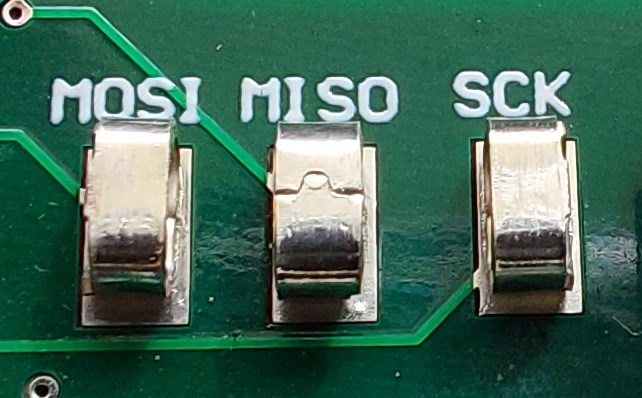
\includegraphics[width=5cm]{../guide/figs/testpoints.jpg}  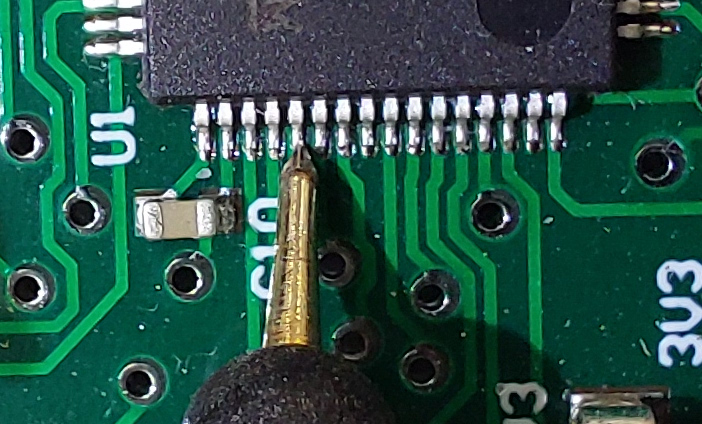
\includegraphics[width=5cm]{../guide/figs/micro_probe_zoom.jpg}

\item Label the test points on the silk screen with meaningful names.

\item Add ground test points that you can clip an oscilloscope ground
  lead to.  Keep these away from other test points to avoid shorting
  with the oscilloscope ground clip.

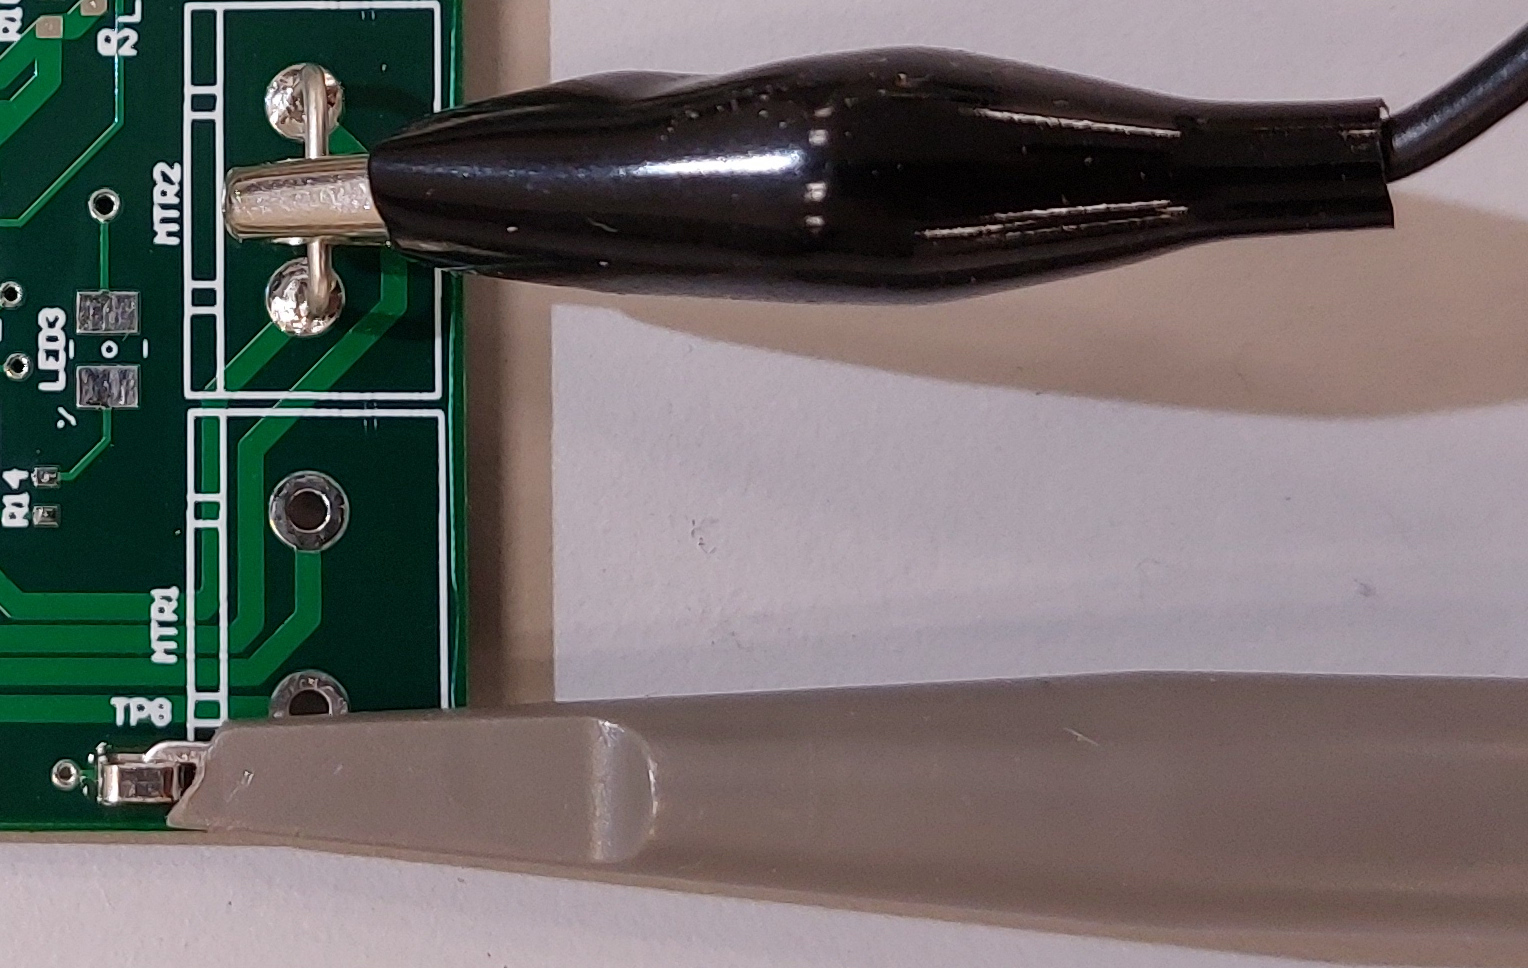
\includegraphics[width=5cm]{figs/scope_probe_testpoints.jpg}

\item Check mounting holes.

\item Check component footprints, especially connectors, voltage
  regulators, and surface mount transistors by placing the parts on a
  print-out of the PCB design.

\item Ensure that power supply traces are wide as possible, preferably
  planes, to reduce their inductance.

\item Ensure that high current traces are wide as possible to reduce their resistance.

\item Do not connect IC pins directly between the pads since it is not
  possible to tell if a solder blob is accidental or deliberate.

\item Insert vias to ground plane to ensure that all parts are connected.  Do not leave unconnected copper.

\item If not using plated through vias do not place vias under
  components.

\item If placing vias under components with exposed metal pads, make
  sure the vias are ``tented'' (covered in solder mask) to prevent
  unexpected shorts.

\item Stitch power or ground planes where vias or tracks cut them up.

\item If a track is of width W it should be separated from the next
  track by a width 2W to reduce crosstalk.  This is the 3-W rule since
  the track centres are 3W.  An exception is for differential signals;
  these should be routed close together with a uniform spacing.

\item Do not run a microstrip traces right on the edge of the PCB.  If
  track is of width W it should be at least W from the edge to reduce
  electric field fringing effects.

\item Use large traces for pads on connectors that may be subject to
  mechanical forces (power jacks, pluggable terminals, etc.) to
  prevent trace cracking.

\item If you have high voltages check clearances.

\item Check pad to track clearances to avoid potential solder bridges.

\item Check that it is possible to top-solder through-hole components
  on non-plated-through boards.

\item Ensure like signals are grouped, data lines, address lines, control lines, analogue signals, etc.

\item Check the thermal path for parts that get hot.

\item Run tracks over reference (power or ground) planes to create a
  microstrip trace; avoid tracks running over cuts in a reference
  plane.

\item Check that hole diameters are larger than the pin diameters for
  connectors and through hole. 25\% over the lead diameters is
  typical.  Remember to look at the diagonal dimension for square pins
  or your holes may be too small.

\item Check the drill file report to make sure the hole sizes are what
  you would expect. There should be no holes with sizes of zero, no
  weird sizes, no super large sizes unless required by the design.

\item Check that connections of thermal vias have clearance to other
  traces and pads.

\item Pay close attention to clearances on internal planes of
  multilayer boards; shorts on these planes can only be removed with
  precision drilling.

\item Number pins on connectors, big ICs, selection jumpers, etc. For
  connectors, number enough pins that pin ordering is obvious. For
  large ICs consider adding tickmarks every 5 pins.

\item Make the pad for pin 1 of every IC square. Also consider putting
  a silkscreen dot next to pin 1.

\item Leave at least 20--50\,mils (0.5--1.3\,mm) clearance between
  components and the edge of the board. This makes it less likely that
  inaccuracies in board fabrication will cause part of a pad to get
  chopped off.

\item Check for component clearances from enclosure including heights.

\item Look at each net individually to ensure that it doesn't take an
  overly long path around the board. Many layout tools have a
  highlight net feature that makes this a fast process.

\item Don't let the silkscreen overlap pads. Try to avoid having
  silkscreen overlapping via holes or areas of the board that will be
  routed away (large holes, slots, tabs, etc.), since legibility will
  be poor.

\item If ICs are being soldered with solder paste ensure that there is
  a solder mask between pads.
 \end{enumerate}



\section{Design rule checks}


This section considers common Altium design rule violations.  For more
information see the Altium wiki.



\subsection{PCB manufacture violations}

You do not want any of these.  If a trace is too thin then etching may
produce a hole in it.  It two traces are too close together, they may
end up joined.


\subsection{PCB assembly violations}


\subsubsection{SMD neck-down constraint}

Traces connecting to SMD pads often need to be reduced in thickness to
minimise heat transfer from the SMD pad (unequal PAD temperatures can
lead to component tombstoning or rotation in the oven).  The traces
widths should be a maximum of 50 \% of the width of the pad and should
be of the same size to prevent component movement due to unequal pad
temperatures.  The length of the neck-down can be as short as 0.5\,mm.

This is not so critical for integrated circuits with many pins (except
if a solder mask is not used since solder might flow away from the
pad).


\subsubsection{Silk to solder mask}

Here Altium thinks the silk screen is being printed over a pad; most
manufacturers detect this and delete the offending text.


\subsubsection{Minimum solder mask sliver constraint}

This occurs with chips having pins that are close together.  It is a
warning that the PCB manufacturer may not be able to make the thin
sliver of solder mask that is applied between pads to reduce the
chances of having a solder blob between the pins.  For a prototype it
is not a concern since the solder blob can be easily removed with a
small soldering iron.


\subsection{Signal integrity violations}

\subsubsection{SMD pad to plane constraint}

What this means is that you have placed a via to a power or ground
plane too far from a SMD pad.  Simply add another via closer to the
pad.  There is no need to skimp on vias for power supply connections.

This violation indicates you that you are adding unnecessary
inductance by increasing the loop area and thus compromising signal
integrity.

Unfortunately, Altium does not detect when you use a power decoupling
capacitor to mitigate this inductance and thus will report
false-positives.  For some reason, whenever there is a decoupling
capacitor pad between an IC pad and a via to a plane, it cannot
calculate the distance of the trace and reports it as being about
2.3\,m!  So, ignore this error.

The goal is to place the decoupling capacitor to minimise the area of
the loop formed by the current flowing from the capacitor to the IC
power and ground pins.  Multiple vias to power/ground planes should
then be placed on the other side of the capacitor.
